\documentclass[stu,12pt]{apa7}
\usepackage{graphicx}
\usepackage{amsmath}
\usepackage{tabularray}
\usepackage{siunitx}
\UseTblrLibrary{siunitx}
\usepackage{float}
\usepackage[american]{babel}
\usepackage{csquotes}

\usepackage[style=apa, backend=biber]{biblatex}
\addbibresource{bibliography.bib}

\title{Beyond Class Voting: Examining the Role of Psycho-Social Antecedents in Political Preferences}
\author{Júlia Quintaneiro Pimenta}
\shorttitle{}
\affiliation{\mbox{Master in the Social Sciences, Universidad Carlos III de Madrid}}
\course{19306: Social Stratification I}
\professor{Héctor Cebolla Boado}
\duedate{28 May 2026}

\abstract{
Pure class voting can be argued to be largely outdated in current times. Although contextual factors have been largely tested, such as educational attainment, individual-level differences have yet to be explored for the most part. As such, it is argued that an individual’s perceived relative deprivation and risk aversion play a role in their political preferences. Additionally, social class is only expected to be involved as a conditioning factor. Through multiple regression and two moderation analyses, it is shown that relative deprivation directly impacts political preferences, leading voters to shift to the political right. In addition, risk aversion is also demonstrated to be associated with right-wing preferences. This is in contrast with previous findings, which suggest that risk-averse individuals should be generally more left-leaning and favour redistribution. Furthermore, social class does not have a conditioning effect on the relationship. The implications of the findings are discussed.
}
\keywords{subjective class perception, left–right voting, political preferences, relative deprivation, risk aversion}

\begin{document}

\maketitle

Class can arguably be seen as one of the largest dividers in a society. It has been the basis for various theories, one of those being theories on voting behaviour. How does a person decide which party to vote for? Does one vote on the basis of economic interests or cultural concerns? Does class play a role in how these are determined? For long, there have been debates on how social class could have an influence on these decisions, and within sociological and political science literature, there have been attempts to discern influential factors that drive or mediate voting outcomes \parencite{PDFSocialClass}.

Within the last decades, the role of social class has shifted. Increasingly, other factors have been argued to play a crucial role, such as education \parencite{hoogheFieldEducationPolitical2025}. However, most recently, there has been a shift to take into account individual-level factors that go beyond one’s class identification or educational attainment, such as identity \parencite{bornschierHowUsThem2021b}. With it, there has been a rise in research on relative deprivation and risk aversion \parencite{cenaRelativeDeprivationNational2023, gartnerIndividualRiskPreferences2017, rooduijnParadoxWellbeingUnfavorable2018a}.

Explanations on the individual or psychological level stand out from other previously examined ones. On the one hand, they are an alternative explanation to structural factors, such as purely class-based theories. Theories focused on those can explain generally why groups differ in political preferences, but not why two individuals within the same group might. Although a certain group has the same material or objective circumstances, the individuals within that group could differ in how they respond to those circumstances. In other words, individual characteristics impact political preferences beyond structural factors.

On the other hand, individual-level factors fill a gap in current research, especially within the field of sociology. Structural factors have been largely the focus, and although they have predictive importance, they ignore characteristics which could drive differences within groups. As such, bridging the gap between the individual-level focus of psychology and the structural factors emphasised in sociology and political science becomes crucial to understand the interdisciplinary nature of political preferences.

Of these, relative deprivation and risk aversion have been partially present in previous literature. Relative deprivation has recently gained newfound importance with rising inequality, and therefore demonstrates clear societal relevance for further research \parencite{rooduijnParadoxWellbeingUnfavorable2018a}. Risk aversion as a predictor taps more into personal characteristics, shown nevertheless to have predictive importance \parencite{oshriRiskAversionGender2023, gartnerIndividualRiskPreferences2017}. To connect these, perceived social class stands out as a classic conditioning factor.

Thus, the following question is investigated: To what extent do perceived relative deprivation and risk aversion influence an individual’s political preferences, and how does perceived social class moderate the effect? First, to examine the question at hand, the literature will be outlined, which, taken together with the proposed mechanisms, will form part of the theoretical framework. Second, the methods for the empirical research as well as the results of the analysis will be presented. Finally, the results and their implications will be discussed and the conclusion drawn.

\section{Theoretical Framework}

\subsection{The Stratification of Political Preferences}

Having outlined the general topic, relevance, and the research question, this section will elaborate on the previously established predictors of political preferences as well as voting outcomes. Historically, voting outcomes have been explained using class as a predictor, arguing that one’s class plays a decisive role, which was termed \textit{class voting} \parencite{PDFSocialClass}. More recent approaches have been distancing themselves from the original class voting scheme. It seems to have only limited predictive capabilities in the context of recent decades.

Before discussing the impact of social class, however, it should be addressed how voting outcomes should be determined, as in, the outcome, as it is also subject to debate. Approaches can be differentiated between voting turnouts, such as which party an individual votes for, and subjective perception, such as a self-placement on a political left–right scale \parencite{lesschaevePredictivePowerLeftright2017}. Additionally, other measures have been proposed that capture the current political arena more accurately than a left–right spectrum, namely the green–alternative–libertarian (GAL) and traditional–authoritarian–nationalist (TAN) dimensions, which are said to be more representative of European politics \parencite{hoogheDoesLeftRight2002a}. Current research uses different outcome measures; they all, however, tie back to political preferences.

\textcite{bengtssonClassIdeologicalOrientations2013a} conducted an analysis linking class position to ideology using a Swedish population sample. The mechanisms through which class impacts ideology were found to be, on the one hand, economic self-interest, which stems from the material conditions, and, on the other hand, education. Work-related factors are also mentioned, which the authors argue should be considered when understanding voting behaviour \parencite{bengtssonClassIdeologicalOrientations2013a}. In other words, it can be argued that class as such is not necessarily a main driver of voting preferences, but rather what it means to be part of a certain class: what material conditions one has, both in terms of income and work, and what education one can obtain.

\textcite{jansenClassVotingLeft2013} observe a general decline in class voting. They find that it is contextual whether there is a decline or not by looking at data from various Western countries in a hierarchical analysis. The more parties are polarised along the left–right axis, the more class voting can be observed in a certain country. More interestingly, they state that education plays a role in how class voting has declined \parencite{jansenClassVotingLeft2013}. All this plays into the idea that class voting is increasingly outdated, and that other factors might play a stronger role.

Another advance in current debates is that it is increasingly stipulated that education is a better predictor of voting outcomes than class. \textcite{hoogheFieldEducationPolitical2025} argue, using the GAL–TAN dimension as the outcome, that education is the single most important predictor for which party an individual chooses to vote. The authors show in a cross-country comparison with 15 European countries that the effect of education is multifaceted. There are impacts from self-selection into education, effects during education, and from the following occupation \parencite{hoogheFieldEducationPolitical2025}.

Another piece to the puzzle is identity. \textcite{bornschierHowUsThem2021b} conduct a survey in Switzerland to analyse the role of identities in the emerging new left and far right. In general, they find that how people vote is not determined solely by policy preferences, such as redistribution, but rather by how they identify. Social structures, such as class and education, drive people to create identities, which in turn impact them ideologically \parencite{bornschierHowUsThem2021b}. It can be argued that identities, in turn, condition how people experience their economic and social reality. In sum, the shift from general class voting to accounting for contextual factors highlights a greater need to address the gap in how these impact political preferences.

\subsection{Relative Deprivation}

It was established that in previous literature, there has been a shift from social class to a stronger focus on other system-level variables which impact voting, as well as individual-level characteristics, such as educational attainment and redistributive preferences. Now, this section will elaborate on psychological or cognitive mechanisms which play a role. Specifically, \textit{relative deprivation} will be discussed, which can be defined as “the perception by an individual that the amount of a desired resource (e.g., money, social status) they have is less than some comparison standard” \parencite{Relative_deprivation}. Particularly, what matters to an individual is not the amount they have, but rather how much they have in comparison with others, and thus how deprived of a particular resource they are.

\textcite{cenaRelativeDeprivationNational2023} show that it is related to right-wing voting for high-income individuals who live in wealthy countries through a multilevel moderated model. In other words, the more an individual feels deprived in relation to others, the more likely they are to vote right, given they belong to a higher social class, operationalised through income \parencite{cenaRelativeDeprivationNational2023}. In a French population sample, \textcite{urbanskaSwayingExtremeGroup2018} find that group relative deprivation is a determinant for voting for the radical right. As such, feeling like one’s in-group—in this case, French people—is left behind can lead to individuals turning to the right.

Going a step further, \textcite{burgoonPositionalDeprivationSupport2019} investigate how left-wing or right-wing voting preferences are impacted by deprivation over time, which is termed \textit{positional deprivation}. Like \textcite{cenaRelativeDeprivationNational2023}, the authors find that it fuels support for radical parties. Specifically, falling behind the wealthiest decile is shown to drive support for the radical left, while falling behind the poorest decile drives support for the radical right. This supplements the findings by \textcite{urbanskaSwayingExtremeGroup2018} by explaining also why some people turn to the radical left, while others to the radical right.

Drawing on the literature, it can be said that relative deprivation seems to impact political preferences through one’s class. In contrast with traditional class voting literature, it is expected that poorer people turn to the right rather than the left, as they feel as if they are being left behind relative to others who might, objectively speaking, be worse off. In terms of cognitive mechanisms, this could be explained through the \textit{Last Place Aversion Paradox}, which hypothesises that, even though it would be beneficial to be in favour of redistribution for a poorer person, they might choose to be against it, as they want to avoid being at the bottom of the income distribution, at the cost of still being badly off \parencite{kuziemkoLastPlaceAversionEvidence2014}.

In sum, there is support that relative deprivation plays a role in political preferences. Although previously untested, there are also indications that social class is an important factor. Specifically, income was shown to condition the relationship \parencite{cenaRelativeDeprivationNational2023}. Thus, drawing on the discussed findings, it is hypothesised that individuals feeling more relatively deprived categorise themselves as more politically right (H\textsubscript{1}), and that higher class positioning strengthens the relationship between relative deprivation and political preferences (H\textsubscript{2}).

\subsection{Risk Aversion}

Having discussed the role of relative deprivation, this section will elaborate on \textit{risk aversion} as a predictor of political preferences, which can, in general, be defined as “the tendency, when choosing between alternatives, to avoid options that entail a risk of loss, even if that risk is relatively small” \parencite{Risk_aversion}. In other words, individuals who show a higher aversion to risk generally do not make choices where the outcome is uncertain. Even if in the long term, taking a more uncertain choice would be more beneficial, the risk-averse individual would not venture it and rather choose something where the outcome is certain. This can then be argued to have an impact on various areas of their life, including their political choices.

\textcite{oshriRiskAversionGender2023} investigate whether risk aversion is what drives the differences between voting in men and women, as men generally tend to vote more right-wing, and women tend to vote left-wing. Through a cross-comparison of 14 countries using public opinion data, they establish that risk-taking might be what drives the gender differences. As women are generally more averse to risk, they vote more left-wing, while men, who are less averse to risk, vote more right-wing \parencite{oshriRiskAversionGender2023}. This has implications beyond gender: If an individual is generally less risk-taking, they might choose not to vote right, irrespective of the gender stratification.

This is further emphasised by \textcite{gartnerIndividualRiskPreferences2017}, who research whether there is a relationship between risk aversion and preferences for redistribution. They do so using available data and administrative records of a sample of the Swedish population. In general, a clear link between risk aversion and the demand for redistribution can be established, which can be argued to explain not only gender stratification, but also age stratification, that is to say, that older people generally favour redistribution while also not being likely to take risks. Interestingly, income is found to have a negative association, meaning that lower-income people prefer redistribution generally more \parencite{gartnerIndividualRiskPreferences2017}.

The effect of class on the link between risk aversion and political preferences is not directly tested by previous literature. \textcite{rooduijnParadoxWellbeingUnfavorable2018a} test the effect of contextual factors on the link between well-being and voting for the radical right or radical left, such as relative deprivation and risk aversion. For risk aversion specifically, they find that voters avoid both radical left and radical right parties if they are generally risk-averse, as voting for extremes is perceived to pose a more significant threat. Additionally, they find that this is mainly true for less well-off citizens, which means they will only vote for radical parties if they find themselves in generally more favourable circumstances \parencite{rooduijnParadoxWellbeingUnfavorable2018a}.

In sum, risk aversion has been shown to be tied to voting for the political left. Additionally, it is linked with a demand for redistribution, which can be seen as ideologically left. Based on the previous literature on risk aversion, and specifically the model by \textcite{rooduijnParadoxWellbeingUnfavorable2018a}, it can also be reasonably concluded that social class could condition the link between risk aversion and political preferences. Thus, it is hypothesised that individuals who are more risk-averse vote more left (H\textsubscript{3}), and that lower class positioning strengthens the relationship between risk aversion and political preferences (H\textsubscript{4}).

\section{Method}

\subsection{Sample and Data}

The sample was drawn from the German General Social Survey (\textit{N} = 2,136; \cite{ackermannGermanGeneralSocial2025}). Of the participants, 49.06\% identify as male (\textit{n} = 1,048), 50.70\% identify as female (\textit{n} = 1,083), and 0.23\% as non-binary (\textit{n} = 5). The participants’ age ranges from 18 to 99 (\textit{M} = 52.62, \textit{SD} = 18.04). From the sample, 1.03\% of the participants completed only pre-primary education (\textit{n} = 22), 16.67\% completed primary education or first stage of basic education (\textit{n} = 356), 31.69\% completed lower secondary or second stage of basic education (\textit{n} = 677), 12.78\% completed secondary or upper secondary education (\textit{n} = 273), 37.22\% completed post-secondary non-tertiary education (\textit{n} = 795), 0.33\% completed first stage of tertiary education (\textit{n} = 7), and 0.28\% completed second stage of tertiary education (\textit{n} = 6).

\subsection{Variables}

The dependent variable (DV) assesses voting choice on the left–right scale. A single item (\textit{pa01}) was used, which asks participants to self-classify their political standing on a scale ranging from 1 (\textit{left}) to 10 (\textit{right}). This is based on the argument by \textcite{lesschaevePredictivePowerLeftright2017} that self-placement is sufficient to assess one’s voting and policy preferences. As such, it was operationalised through a single item.

The two predictors are relative deprivation and risk aversion. The first independent variable (IV) asks whether the participant feels like they are getting their fair share (\textit{id01}), ranging from 1 (\textit{much less}) to 4 (\textit{more than a fair share}). The second IV asks whether they strive to avoid risks (\textit{vg10}), ranging from 1 (\textit{not at all}) to 6 (\textit{extremely}). They are expected to operationalise the level of relative deprivation and risk aversion of the participants, respectively. The moderator is subjective class classification (\textit{id02}), ranging from 1 (\textit{lower class}) to 5 (\textit{upper class}). Four control variables were chosen to improve model fit. The variables selected are gender (\textit{sex}), age (\textit{age}), education level (\textit{educ}), and income (\textit{incc}).

\subsection{Procedure}

This study employs a cross-sectional research design using secondary survey data. In general, the data were cleaned of all missing values and whenever a response was refused. Three ordinary least squares (OLS) regression models were estimated using political left–right placement as the DV. For the first model, relative deprivation and risk aversion were the selected IVs to see the main effect:
\[pa01_i=\beta_0+\beta_1id01_i+\beta_2vg10_i+\beta_3sex_i+\beta_4age_i+\beta_5educ_i+ \beta_6incc_i+ \varepsilon_i\]
For the second model, relative deprivation was moderated by class:
\[pa01_i=\beta_0+\beta_1(id01 \times id02)_i+\beta_2sex_i+\beta_3age_i+\beta_4educ_i+\beta_5incc_i+  \varepsilon_i\]
The third model moderated class on risk aversion:
\[pa01_i=\beta_0+\beta_1(vg10 \times id02)_i+\beta_2sex_i+\beta_3age_i+\beta_4educ_i+ \beta_5incc_i+\varepsilon_i\]
All models control for gender, age, education, and income, and use robust standard errors following significant Breusch–Pagan tests for all three models, \textit{BP}(6) = 22.64, \textit{p} < .001, \textit{BP}(7) = 21.86, \textit{p} = 0.0027, and \textit{BP}(7) = 18.21, \textit{p} = 0.011, respectively. Additionally, the variables \textit{id02} and \textit{id01} were mean-centred for the interaction effects following high variance inflation factors. The detailed analysis and full diagnostics are available in the supplementary repository \parencite{zotero-item-1650}.

\section{Results}

\subsection{Main Effect}

An OLS regression was run to test the effect of relative deprivation and risk aversion on political left–right placement. The overall model was statistically significant, explaining 5.42\% of the variance in political preferences, \textit{R}\textit{\textsuperscript{2}} = .054, \textit{F}(6, 2129) = 20.33, \textit{p} < .001. Relative deprivation showed a negative and significant effect, meaning that people who perceive themselves as less deprived are predicted to vote more left-leaning, \textit{b} = -0.23, \textit{SE} = 0.055, \textit{t} = -4.19, \textit{p} < .001. The effect of risk aversion was positive and significant, indicating that more risk-averse participants are predicted to vote more right, \textit{b} = 0.068, \textit{SE} = 0.033, \textit{t} = 2.07, \textit{p} = .039. The main effects are plotted in Figure 1.

\begin{figure}
    \centering
    \caption{Main Effects}
    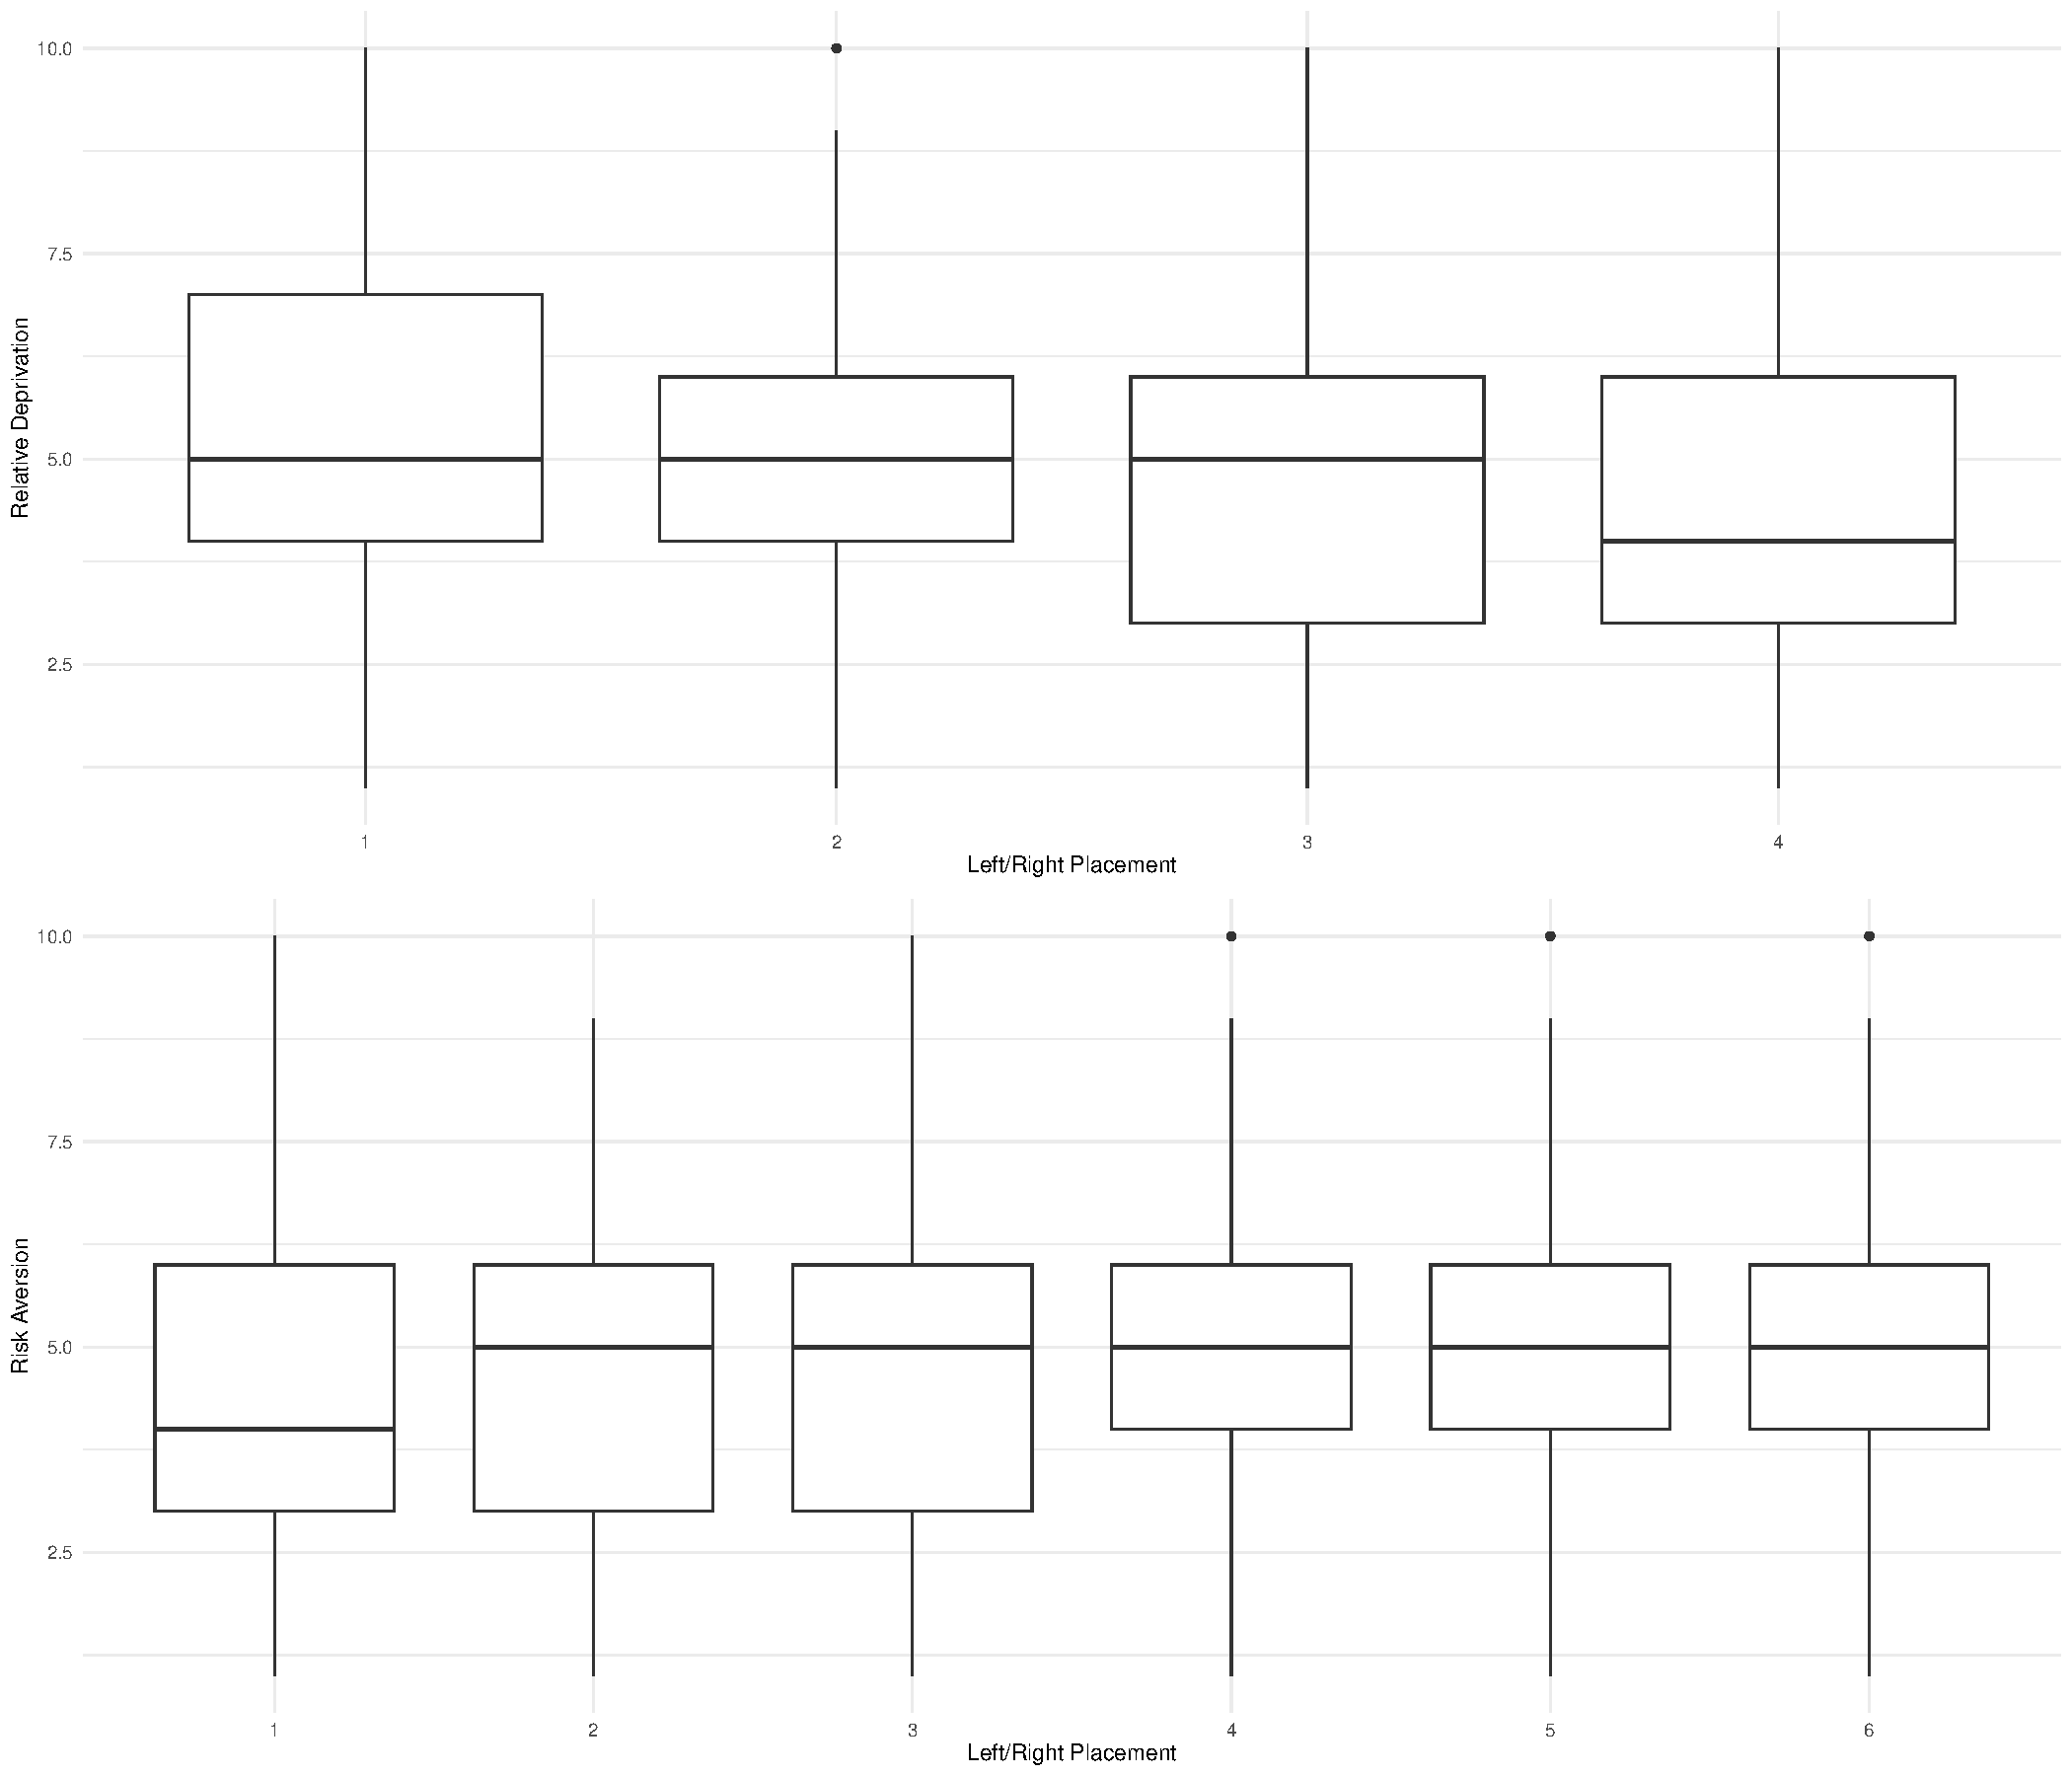
\includegraphics[width=1\textwidth]{figures/main.pdf}
\end{figure}

\subsection{Interaction Effects}

Two OLS regressions were run to estimate whether subjective class placement moderates relative deprivation and risk aversion, using political left–right placement as the outcome. For relative deprivation, the model was significant, explaining 5.71\% of the variance, \textit{R}\textit{\textsuperscript{2}} = .057, \textit{F}(7, 2128) = 18.39, \textit{p} < .001. Class was shown to positively and non-significantly interact with the predictor, \textit{b} = 0.023, \textit{SE} = 0.065, \textit{t} = 0.35, \textit{p} = .72. For risk aversion, the model was significant, explaining 4.70\% of the variance, \textit{R}\textit{\textsuperscript{2}} = .047, \textit{F}(7, 2128) = 15.01, \textit{p} < .001. The interaction was also positive and non-significant, \textit{b} = 0.039, \textit{SE} = 0.043, \textit{t} = 0.92, \textit{p} = .36. The interaction plots can be found in Figure 2. Table 1 summarises the results of all three models.

\begin{figure}
    \centering
    \caption{Interaction Effects}
    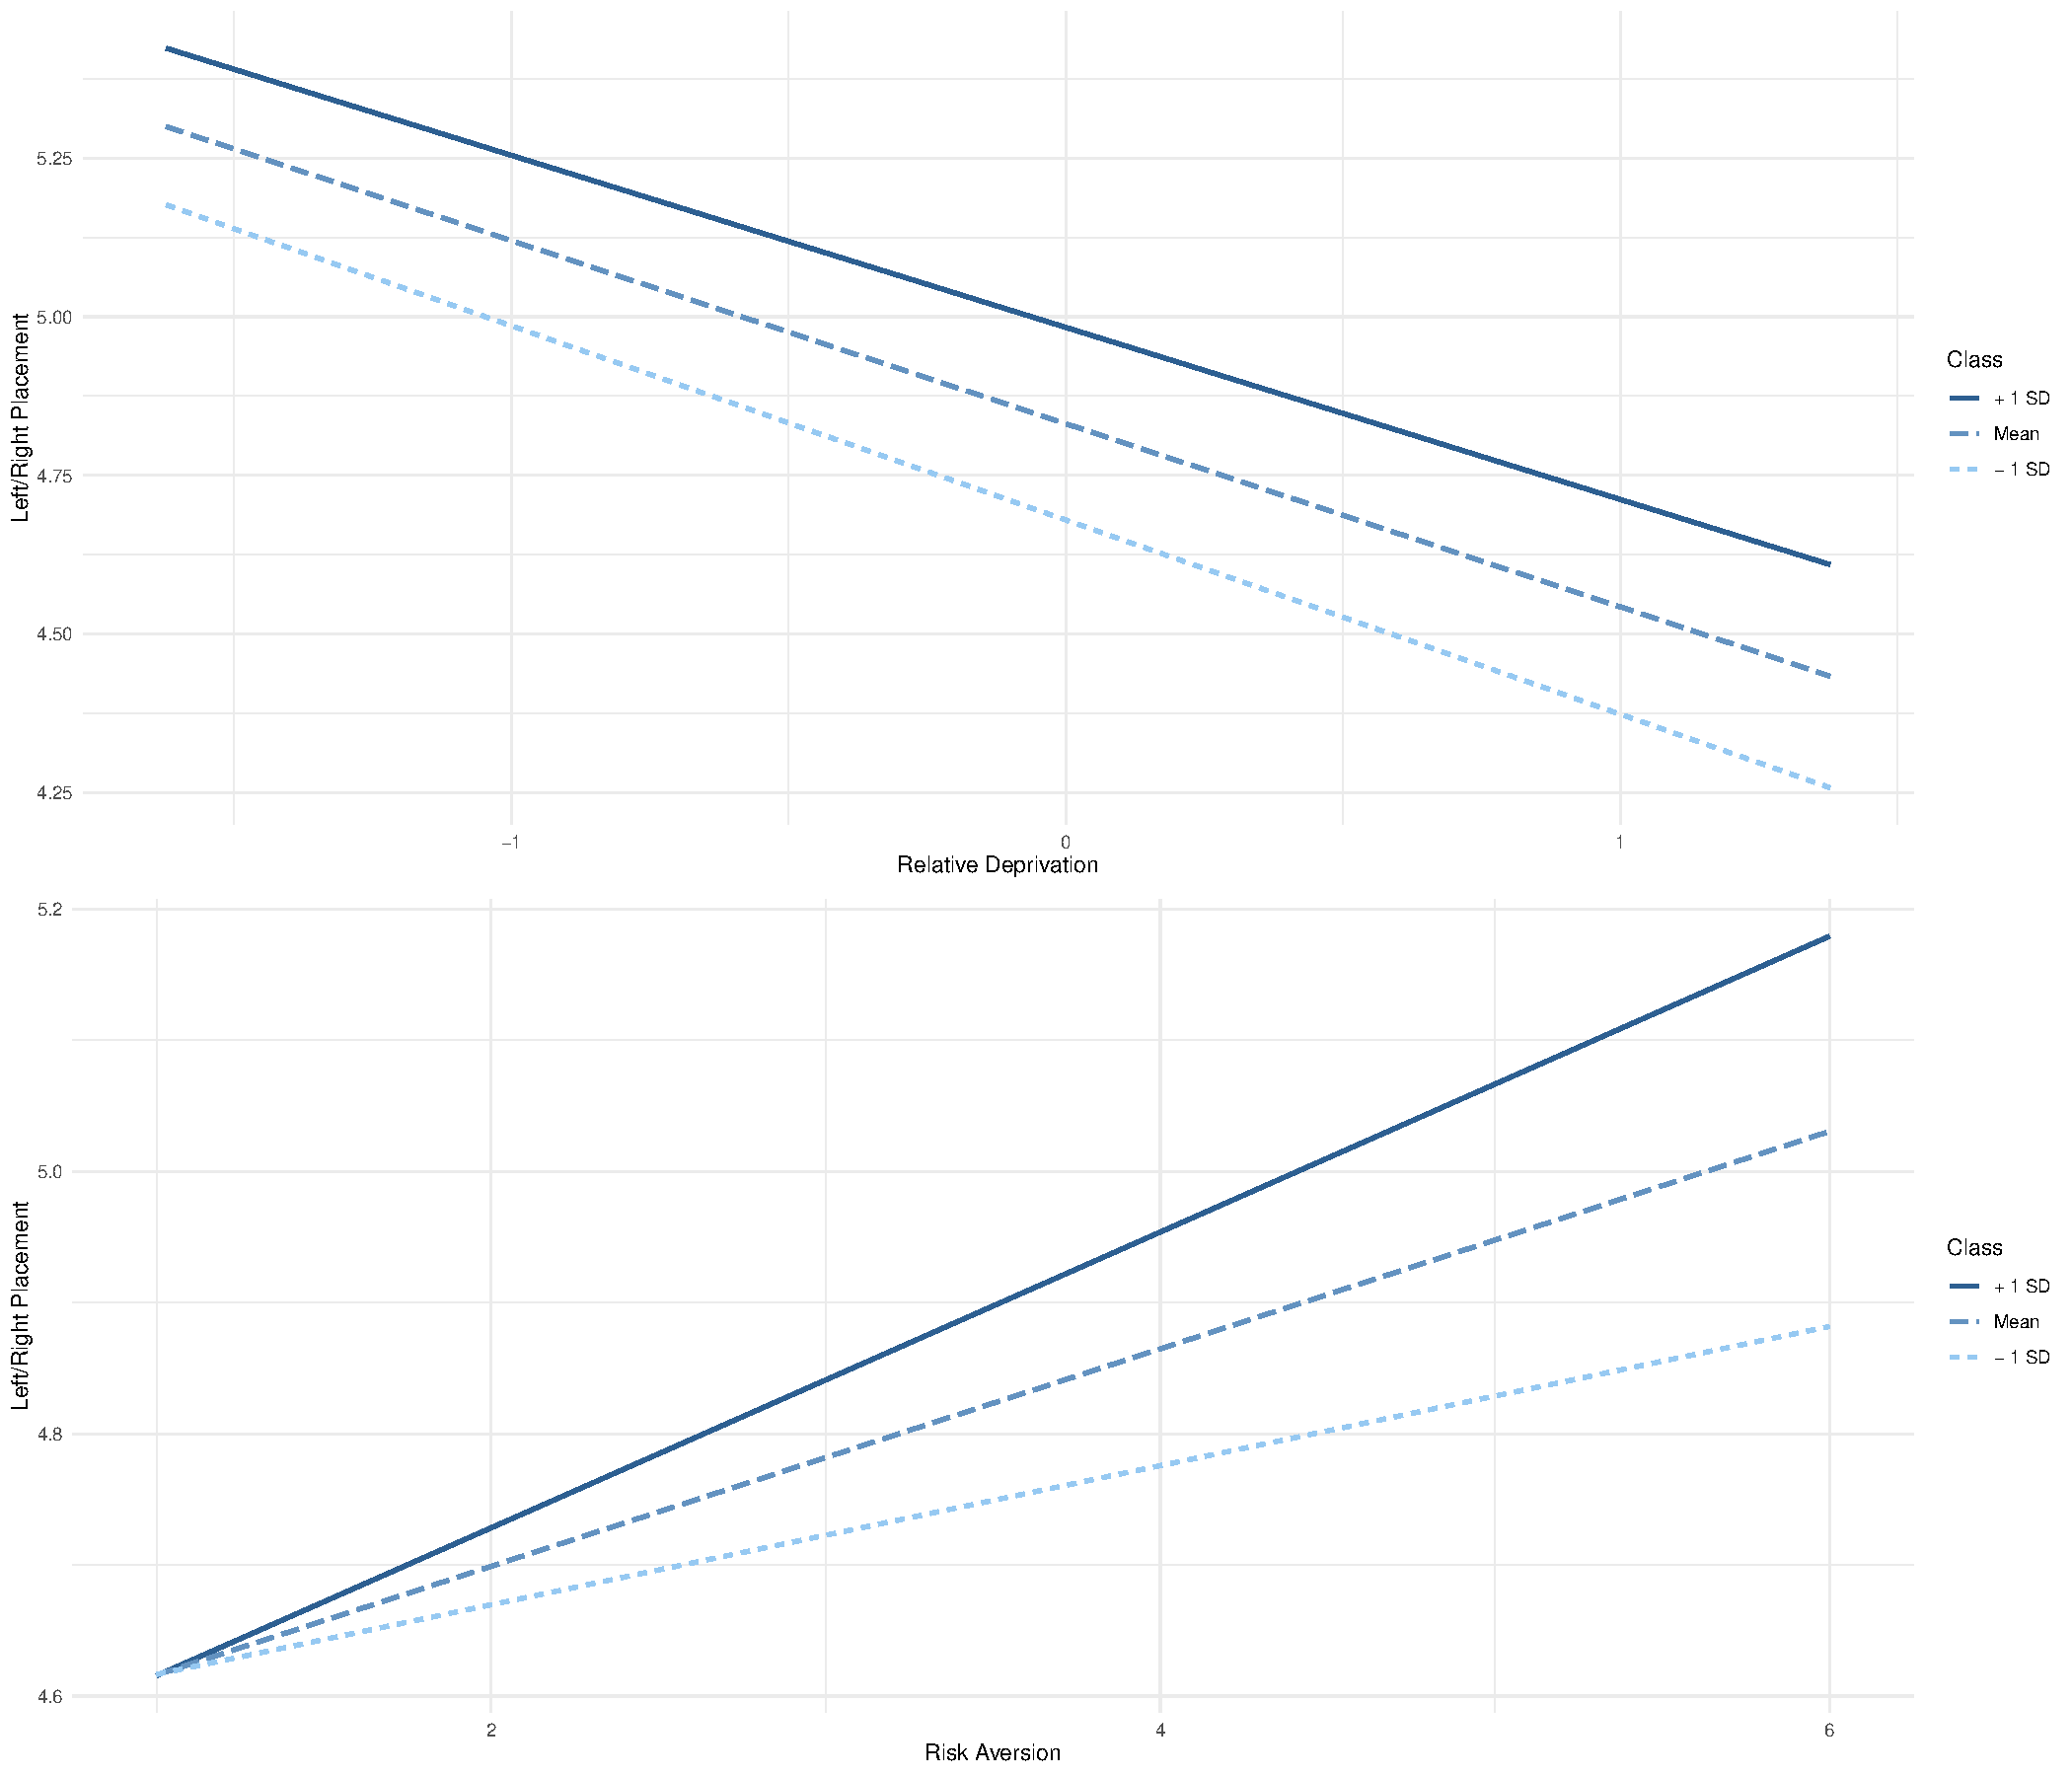
\includegraphics[width=1\textwidth]{figures/inter.pdf}
\end{figure}

\begin{table}
\caption{Coefficients}
\centering
\scalebox{0.65}{%
\begin{talltblr}[         %% tabularray outer open
entry=none,label=none,
note{}={+ p \num{< 0.1}, * p \num{< 0.05}, ** p \num{< 0.01}, *** p \num{< 0.001}},
]                     %% tabularray outer close
{                     %% tabularray inner open
colspec={Q[]Q[]Q[]Q[]},
hline{2}={1-4}{solid, black, 0.05em},
hline{24}={1-4}{solid, black, 0.05em},
hline{1}={1-4}{solid, black, 0.08em},
hline{33}={1-4}{solid, black, 0.08em},
column{2-4}={}{halign=c},
column{1}={}{halign=l},
}                     %% tabularray inner close
& Main & Interaction (Relative Deprivation) & Interaction (Risk Aversion) \\
(Intercept) & \num{6.276}*** & \num{6.280}*** & \num{6.027}*** \\
& (\num{0.312}) & (\num{0.273}) & (\num{0.312}) \\
Relative Deprivation & \num{-0.232}*** &  &  \\
& (\num{0.055}) &  &  \\
Risk Aversion & \num{0.068}* &  & \num{0.083}* \\
& (\num{0.033}) &  & (\num{0.033}) \\
Sex & \num{-0.374}*** & \num{-0.396}*** & \num{-0.382}*** \\
& (\num{0.079}) & (\num{0.079}) & (\num{0.080}) \\
Age & \num{-0.002} & \num{-0.002} & \num{-0.003} \\
& (\num{0.002}) & (\num{0.002}) & (\num{0.002}) \\
Education & \num{-0.227}*** & \num{-0.270}*** & \num{-0.276}*** \\
& (\num{0.039}) & (\num{0.040}) & (\num{0.040}) \\
Income & \num{0.028}*** & \num{0.017}+ & \num{0.018}* \\
& (\num{0.009}) & (\num{0.009}) & (\num{0.009}) \\
Relative Deprivation, centred &  & \num{-0.289}*** &  \\
&  & (\num{0.058}) &  \\
Class, centred &  & \num{0.200}** & \num{-0.040} \\
&  & (\num{0.065}) & (\num{0.177}) \\
Relative Deprivation, centred × Class, centred &  & \num{0.023} &  \\
&  & (\num{0.065}) &  \\
Risk Aversion × Class, centred &  &  & \num{0.039} \\
&  &  & (\num{0.043}) \\
Num.Obs. & \num{2136} & \num{2136} & \num{2136} \\
R2 & \num{0.054} & \num{0.057} & \num{0.047} \\
R2 Adj. & \num{0.052} & \num{0.054} & \num{0.044} \\
AIC & \num{8446.6} & \num{8442.1} & \num{8464.6} \\
BIC & \num{8491.9} & \num{8493.1} & \num{8515.6} \\
Log.Lik. & \num{-4215.284} & \num{-4212.040} & \num{-4223.321} \\
F & \num{20.188} & \num{17.944} & \num{14.693} \\
RMSE & \num{1.74} & \num{1.74} & \num{1.75} \\
Std.Errors & HC3 & HC3 & HC3 \\
\end{talltblr}%
}
\end{table}


\section{Discussion}

In the previous section, it was tested whether relative deprivation and risk aversion have an effect on an individual’s political left–right placement, and whether subjective class placement moderates the effect. In the following, the results will be discussed in light of the literature. First, a significant effect was found for both relative deprivation and risk aversion. Specifically, it was found that individuals who feel more deprived and are more averse to risk are more likely to categorise themselves as right-wing, which provides support for H\textsubscript{1}, but not for H\textsubscript{3}. Second, none of the interactions had a significant effect. In light of this, it is also dubious to interpret the directionality. As such, H\textsubscript{2} and H\textsubscript{4} cannot be accepted.

The link between relative deprivation and voting for the political right, which has been previously established, could be confirmed \parencite{cenaRelativeDeprivationNational2023, burgoonPositionalDeprivationSupport2019, urbanskaSwayingExtremeGroup2018}. This shows that non-structural factors, or factors that go beyond the traditional class voting, contribute to a person’s political preferences. This also shows that the comparison is likely to be horizontal. One might objectively not be well-off, but rather than compare themselves to the absolute, they compare themselves relatively to others, such as immigrants \parencite{urbanskaSwayingExtremeGroup2018}. This relative comparison is what creates the paradox: Voters shift to the right, which might be against their interests, because of their perceived relative standing.

A possible explanation for the positive relationship between risk aversion and political preferences could be the rise of identity politics, as described by \textcite{bornschierHowUsThem2021b}. Previous findings on risk aversion highlight that risk-averse individuals are drawn to redistributive preferences, but that does not necessarily translate to the current left–right divide \parencite{gartnerIndividualRiskPreferences2017}. As argued by \textcite{hoogheDoesLeftRight2002a}, current European politics fall increasingly under the GAL–TAN umbrella, which deals more with the identitarian side of politics.

There is also evidence that risk-averse individuals are more drawn to the status quo, which could translate in the context of German politics to voting more conservatively \parencite{schwaningerRiskPreferencesDelegation2024}. In other words, risk aversion could not necessarily be tied to voting for the radical right, but rather the moderate, conservative right, which is then reflected in the model. Risk aversion has also been shown to be more predictive of whether a person votes for extremes, such as the radical left or the radical right \parencite{rooduijnParadoxWellbeingUnfavorable2018a}. Rather than being linearly associated with political preferences, it could be a dampening factor for radicalisation.

As for the interaction effects, none could be confirmed. A possible explanation is that the chosen variable did not accurately operationalise social class. For instance, participants could have experienced a central tendency bias, meaning that most perceived themselves as middle class. This is a reported phenomenon: Most people, irrespective of whether they are objectively lower or higher class, for instance in terms of income, would consider themselves to be in the middle \parencite{kulicMisperceptionsIndividualPosition}. Another explanation is that social class simply does not have an effect on whether the link between relative deprivation or risk aversion and political preferences is stronger or weaker.

Instead of social class, there could be other factors conditioning the relationship. For instance, education was consistently tested to have an effect on voting outcomes, and might be more representative of actual class positioning rather than a subjective social class measure \parencite{gethinBrahminLeftMerchant2022, simonExplainingEducationalDivide2022}. Additionally, it has been argued that education is increasingly more important to understand voter stratification than simply class \parencite{gethinBrahminLeftMerchant2022, hoogheHowDoesEducation2026}. In sum, both relative deprivation and risk aversion are associated with a preference for the political right. Social class has been shown not to condition the relationship, which further emphasises the need to think beyond the classic class voting theories.

Some important limitations need to be taken into account. First, the sample was exclusively German, which limits the external validity of the results. The German political landscape might be generalisable to other Western European countries, but remains unique. Future research should consider cross-country comparisons to further strengthen the findings. Second, although the results were significant, the models showed a low fit. This suggests that there are other factors which should be controlled for, for which the current models have not. Future research should include other control variables.

Generally speaking, further research could build on the idea of psycho-social factors influencing political stratification, going beyond the two tested predictors. For example, the link between personality and voting outcomes could be further tested. Moreover, future research could test whether personal characteristics are what drive people to vote differently when part of the same social group. This is also highly societally relevant, as it could be used as a basis to assess what propels people to vote radically, and therefore also how to mitigate the individual factors that might do so. Beyond that, further research could test education as a conditioning factor rather than a direct predictor of political preferences. As argued previously, education could be seen as having largely replaced class voting in current times, which accentuates the need to investigate it further.

\section{Conclusion}

In conclusion, relative deprivation and risk aversion have an effect on political preferences. While relative deprivation has a negative effect, indicating that less deprived individuals are expected to vote more for the political right, risk aversion has a positive effect, meaning that less risk-averse individuals vote more for the political left. The former finding aligns with previous literature, while the latter does not. A possible explanation discussed is that there has been a shift in what political right and political left mean; the shift from redistributive preferences to identity politics could be explanatory for this result. Social class was furthermore found to not have a conditioning effect on the relationship, which further highlights the need to leave class voting in the past. For further research, it is recommended that education as a moderator, as well as other individual-level factors, be considered, so that the disciplinary bridge between psychological and sociological research on political preferences can be surpassed.

\printbibliography

\end{document}
